\documentclass[]{article}
\usepackage{lmodern}
\usepackage{amssymb,amsmath}
\usepackage{ifxetex,ifluatex}
\usepackage{fixltx2e} % provides \textsubscript
\ifnum 0\ifxetex 1\fi\ifluatex 1\fi=0 % if pdftex
  \usepackage[T1]{fontenc}
  \usepackage[utf8]{inputenc}
\else % if luatex or xelatex
  \ifxetex
    \usepackage{mathspec}
  \else
    \usepackage{fontspec}
  \fi
  \defaultfontfeatures{Ligatures=TeX,Scale=MatchLowercase}
\fi
% use upquote if available, for straight quotes in verbatim environments
\IfFileExists{upquote.sty}{\usepackage{upquote}}{}
% use microtype if available
\IfFileExists{microtype.sty}{%
\usepackage{microtype}
\UseMicrotypeSet[protrusion]{basicmath} % disable protrusion for tt fonts
}{}
\usepackage[margin=1in]{geometry}
\usepackage{hyperref}
\hypersetup{unicode=true,
            pdfborder={0 0 0},
            breaklinks=true}
\urlstyle{same}  % don't use monospace font for urls
\usepackage{longtable,booktabs}
\usepackage{graphicx,grffile}
\makeatletter
\def\maxwidth{\ifdim\Gin@nat@width>\linewidth\linewidth\else\Gin@nat@width\fi}
\def\maxheight{\ifdim\Gin@nat@height>\textheight\textheight\else\Gin@nat@height\fi}
\makeatother
% Scale images if necessary, so that they will not overflow the page
% margins by default, and it is still possible to overwrite the defaults
% using explicit options in \includegraphics[width, height, ...]{}
\setkeys{Gin}{width=\maxwidth,height=\maxheight,keepaspectratio}
\usepackage[normalem]{ulem}
% avoid problems with \sout in headers with hyperref:
\pdfstringdefDisableCommands{\renewcommand{\sout}{}}
\IfFileExists{parskip.sty}{%
\usepackage{parskip}
}{% else
\setlength{\parindent}{0pt}
\setlength{\parskip}{6pt plus 2pt minus 1pt}
}
\setlength{\emergencystretch}{3em}  % prevent overfull lines
\providecommand{\tightlist}{%
  \setlength{\itemsep}{0pt}\setlength{\parskip}{0pt}}
\setcounter{secnumdepth}{0}
% Redefines (sub)paragraphs to behave more like sections
\ifx\paragraph\undefined\else
\let\oldparagraph\paragraph
\renewcommand{\paragraph}[1]{\oldparagraph{#1}\mbox{}}
\fi
\ifx\subparagraph\undefined\else
\let\oldsubparagraph\subparagraph
\renewcommand{\subparagraph}[1]{\oldsubparagraph{#1}\mbox{}}
\fi

%%% Use protect on footnotes to avoid problems with footnotes in titles
\let\rmarkdownfootnote\footnote%
\def\footnote{\protect\rmarkdownfootnote}

%%% Change title format to be more compact
\usepackage{titling}

% Create subtitle command for use in maketitle
\newcommand{\subtitle}[1]{
  \posttitle{
    \begin{center}\large#1\end{center}
    }
}

\setlength{\droptitle}{-2em}
  \title{}
  \pretitle{\vspace{\droptitle}}
  \posttitle{}
  \author{}
  \preauthor{}\postauthor{}
  \date{}
  \predate{}\postdate{}


\begin{document}

{
\setcounter{tocdepth}{3}
\tableofcontents
}
\subsection{Informații generale}\label{informatii-generale}

\begin{center}\rule{0.5\linewidth}{\linethickness}\end{center}

Acest curs reprezintă o introducere în teoria probabilităților și a
statisticii matematice. Pentru parcurgerea acestui curs nu sunt necesare
cunoștinte de teoria măsurii.

\begin{center}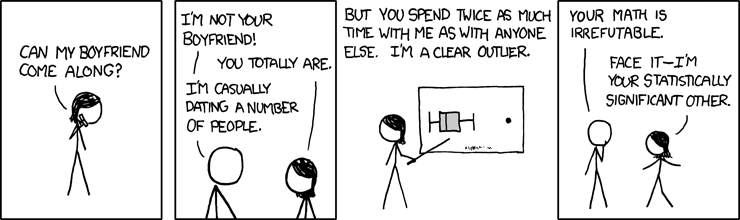
\includegraphics[width=0.8\linewidth]{images/boyfriend} \end{center}

\subsection{Informații de contact}\label{informatii-de-contact}

\begin{center}\rule{0.5\linewidth}{\linethickness}\end{center}

\subsubsection{Curs}\label{curs}

\begin{itemize}
\item
  \emph{Instructor} : \href{https://alexamarioarei.github.io/}{Alexandru
  Amărioarei}
\item
  \emph{Email} : alexandru {[}dot{]} amarioarei {[}at{]} fmi {[}dot{]}
  unibuc {[}dot{]} ro
\item
  \emph{Orar} : Joi 16:00 - 18:00
\item
  \emph{Sala} : Amfiteatrul Pompeiu (Etaj 2) - Seria 24
\end{itemize}

\subsubsection{Seminar/Laborator}\label{seminarlaborator}

\begin{itemize}
\item
  \emph{Instructor} : \href{https://alexamarioarei.github.io/}{Alexandru
  Amărioarei}
\item
  \emph{Email} : alexandru {[}dot{]} amarioarei {[}at{]} fmi {[}dot{]}
  unibuc {[}dot{]} ro
\end{itemize}

\subsection{Note de laborator}\label{note-de-laborator}

\begin{center}\rule{0.5\linewidth}{\linethickness}\end{center}

Mai jos găsiți o parte din laboratoarele cursului.

\begin{longtable}[]{@{}cccc@{}}
\toprule
Nr & Laborator & HTML & PDFs\tabularnewline
\midrule
\endhead
1 & Laborator 1 & \href{labs/Lab_1.html}{HTML} &
\href{labs/Lab_1_pdf.pdf}{PDF}\tabularnewline
2 & Laborator 2 & \href{labs/Lab_2.html}{HTML} &
\href{labs/Lab_2.pdf}{PDF}\tabularnewline
3 & Laborator 3 & \href{labs/Lab_3.html}{HTML} &
\href{labs/Lab_3.pdf}{PDF}\tabularnewline
4 & Laborator 4 & \href{labs/Lab_4.html}{HTML} &
\href{labs/Lab_4.pdf}{PDF}\tabularnewline
5 & Laborator 5 & \href{labs/Lab_5.html}{HTML} &
\href{labs/Lab_5.pdf}{PDF}\tabularnewline
\bottomrule
\end{longtable}

\subsection{Notarea}\label{notarea}

\begin{center}\rule{0.5\linewidth}{\linethickness}\end{center}

Notarea se va face după cum urmează: teme (30\%) distribuite în mod
egal, proiect de laborator (20\%) și examen final (50\%).

\[
  T = \min\left(1+0.5\times E + 0.2\times P + 0.05\times\sum_{i=1}^{6}T_i, 10\right)
\]

\subsection{Teme}\label{teme}

\begin{center}\rule{0.5\linewidth}{\linethickness}\end{center}

Vor fi 6 teme și acestea vor fi postate (aproape) din două în două
săptămâni (de obicei Duminică seara). Este încurajată colaborarea între
studenți dar fiecare student trebuie să își scrie propriile soluții.
Copierea temei este \textbf{interzisă}.

\begin{longtable}[]{@{}ccc@{}}
\toprule
Tema & Data de predare & Solutii\tabularnewline
\midrule
\endhead
\href{homework/Tema1.pdf}{Tema 1} & 21 Octombrie &
\href{homework/Tema1_Sol.pdf}{Solutie Tema 1}\tabularnewline
\href{homework/Tema2.pdf}{Tema 2} & \sout{4 Noiembrie} 6 Noiembrie &
\href{homework/Tema2_Sol.pdf}{Solutie Tema 2}\tabularnewline
\href{homework/Tema3.pdf}{Tema 3} & \sout{20 Noiembrie} 26 Noiembrie &
Solutie Tema 3\tabularnewline
Tema 4 & -- & Solutie Tema 4\tabularnewline
Tema 5 & -- & Solutie Tema 5\tabularnewline
Tema 6 & -- & Solutie Tema 6\tabularnewline
\bottomrule
\end{longtable}

Trimiterea temelor se poate face pe adresa de \textbf{Dropbox} (conform
instrucțiunilor de la curs) până la \emph{data de predare} din tabel,
cel târziu până la ora 23:59.

Studenții trebuie să trimită temele în folderele cu grupele
corespunzătoare. Fiecare temă va fi trimisă în format \textbf{PDF}
(lizibil) iar fișierul va avea numele:
\emph{Tema\_x\_Nume\_Prenume\_grupa\_y.pdf}, unde \emph{x} este numărul
temei iar \emph{y} este numărul grupei.

\begin{rmdcaution}
În cazul în care o temă nu va fi predată la timp, nu va avea formatul
specificat sau nu va fi lizibilă, aceasta va fi punctată cu 0 puncte.
\end{rmdcaution}

\begin{quote}
\textbf{TABELE STATISTICE} Vizualizați tabelele în format
\href{tables/Tabele_Statistice.html}{HTML} sau
\href{tables/Tabele_Statistice_v2.pdf}{PDF}.
\end{quote}

\subsection{Proiect de laborator}\label{proiect-de-laborator}

\begin{center}\rule{0.5\linewidth}{\linethickness}\end{center}

Mai jos găsiți proiectele de laborator pentru cursul de
\emph{Probabilități și Statistică}. Proiectele sunt individuale iar
copierea proiectelor este \textbf{strict interzisă}.

\begin{longtable}[]{@{}ccc@{}}
\toprule
Grupa & Proiect Nr. & Data de predare\tabularnewline
\midrule
\endhead
241, 242, 243, 244 & Proiect 1 & --\tabularnewline
\bottomrule
\end{longtable}

Trimiterea proiectelor se va face pe adresa de \textbf{Dropbox} (conform
instrucțiunilor de la curs) până la \emph{data de predare} din tabel,
dar cel târziu până la ora 23:59.

Studenții trebuie să trimită proiectele în folderele cu grupele
corespunzătoare. Fiecare proiect va fi trimis în format \textbf{PDF} sau
\textbf{MSWord} și va fi generat cu ajutorul pachetului
\href{http://rmarkdown.rstudio.com/index.html}{Rmarkdown} pentru
documente reproductibile. Fișierul final va conține și codul \texttt{R}
(documentat) și va avea numele:
\emph{Proiect\_Nume\_Prenume\_grupa\_x.pdf}, unde \emph{x} este numărul
grupei.

\subsection{Rezultate}\label{rezultate}

\begin{center}\rule{0.5\linewidth}{\linethickness}\end{center}

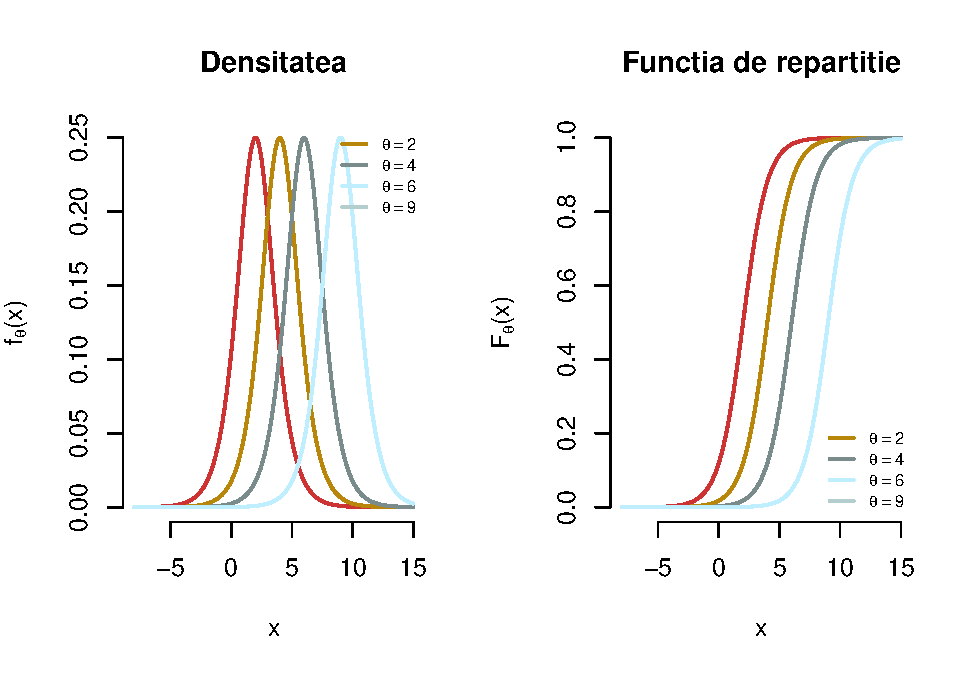
\includegraphics{Probabilitati_Statistica_2017_2018_files/figure-latex/unnamed-chunk-7-1.pdf}

\subsection{Bibliografie}\label{bibliografie}

\begin{center}\rule{0.5\linewidth}{\linethickness}\end{center}

\begin{enumerate}
\def\labelenumi{\arabic{enumi}.}
\tightlist
\item
  Cristian Niculescu - \emph{Probabilități și statistică}, Ed. Univ.
  Buc.
\item
  Dominique Foata, Aime Fuchs - \emph{Calcul des probabilites}, Ed.
  Dunod Paris
\item
  Sheldon Ross - \emph{Introductory statistics}
\item
  Geoffrey Grimmett, David Stirzaker - \emph{Probability and Random
  Processes}
\item
  John Rice - \emph{Mathematical Statistics and Data Analysis}, Duxbury
\end{enumerate}

\subsection{Link-uri utile}\label{link-uri-utile}

\begin{center}\rule{0.5\linewidth}{\linethickness}\end{center}

\subsubsection{R}\label{r}

\begin{enumerate}
\def\labelenumi{\arabic{enumi}.}
\tightlist
\item
  Programul R - \href{https://cran.r-project.org/}{CRAN}
\item
  Interfața grafică \href{https://www.rstudio.com/}{RStudio}
\item
  Documentație R (în engleză) -
  \href{https://cran.r-project.org/doc/manuals/r-release/R-intro.pdf}{R-Intro}
\item
  Documentație R (în română) -
  \href{ftp://cran.r-project.org/pub/R/doc/contrib/Paradis-rdebuts_RO.pdf}{R
  pentru începători}
\item
  Documentație R (în română) -
  \href{http://www.edumanager.ro/community/documente/initiere_in_r.pdf}{Inițiere
  în R pentru persoane cu pregătire matematică}
\end{enumerate}

\subsubsection{Latex}\label{latex}

\begin{enumerate}
\def\labelenumi{\arabic{enumi}.}
\tightlist
\item
  Introducere în Latex (în romană) -
  \href{https://ro.wikibooks.org/wiki/LaTeX_(carte)}{Manual Wikibooks}
\item
  Introducere în Latex (în engleză) -
  \href{https://en.wikibooks.org/wiki/LaTeX}{Wikibooks Latex Manual} în
  special secțiunile de
  \href{https://en.wikibooks.org/wiki/LaTeX/Mathematics}{matematică},
  \href{https://en.wikibooks.org/wiki/LaTeX/List_Structures}{liste},
  \href{https://en.wikibooks.org/wiki/LaTeX/Importing_Graphics}{grafice}
  și
  \href{https://en.wikibooks.org/wiki/LaTeX/Floats,_Figures_and_Captions}{figuri}
\item
  Tutoriale Latex (în engleză) -
  \href{https://www.youtube.com/playlist?list=PLDD406480D35CE390}{video}
\item
  Editoarele:
  \href{http://www.xm1math.net/texmaker/download.html}{Texmaker} și
  \href{http://www.texniccenter.org/}{TeXnicCenter}
\item
  Mediul latex \href{https://miktex.org/}{MiKTeX}
\end{enumerate}

\subsubsection{Rmarkdown}\label{rmarkdown}

\begin{enumerate}
\def\labelenumi{\arabic{enumi}.}
\tightlist
\item
  Pachetul \href{http://rmarkdown.rstudio.com/index.html}{Rmarkdown}
  pentru documente reproductibile
\end{enumerate}


\end{document}
